\documentclass[12pt,letterpaper]{article}

\usepackage[T1]{fontenc}
\usepackage[utf8]{inputenc}

\usepackage[letterpaper,margin=1in]{geometry}
\usepackage{parskip}
\usepackage{ragged2e}
\usepackage[expansion=false]{microtype}

\usepackage{graphicx}
\usepackage{float}
\graphicspath{{./}}

\usepackage{array}
\usepackage{tabularx}
\usepackage{booktabs}
\usepackage[font=small,labelfont=bf,skip=8pt]{caption}

\usepackage{xcolor}
\usepackage{fancyvrb}

\usepackage{titlesec}
\usepackage{mdframed}
\usepackage[colorlinks=true,
            linkcolor=linknavy,
            urlcolor=linknavy,
            citecolor=linknavy,
            pdftitle={TOETAE SPECIAL},
            pdfauthor={John Derby},
            pdfsubject={API documentation}]{hyperref}

\definecolor{linknavy}{HTML}{1A4D8F}
\definecolor{rulegray}{HTML}{8A9199}
\definecolor{notegray}{HTML}{F2F3F5}
\definecolor{notebar}{HTML}{6B7280}

\titleformat{\section}
  {\normalfont\Large\bfseries}{\thesection}{0.75em}{}
  [\vspace{2pt}\titlerule]
\titleformat{\subsection}
  {\normalfont\large\bfseries}{\thesubsection}{0.75em}{}
\titlespacing*{\section}{0pt}{0pt}{12pt}
\titlespacing*{\subsection}{0pt}{16pt}{6pt}

\newcommand{\sectionbreak}{\clearpage}

\DefineVerbatimEnvironment{code}{Verbatim}{%
  fontsize=\small,
  frame=leftline,
  framerule=1.2pt,
  rulecolor=\color{rulegray},
  framesep=10pt,
  xleftmargin=12pt,
  samepage=true%
}

\newmdenv[
  linewidth=2pt,
  linecolor=notebar,
  topline=false, bottomline=false, rightline=false,
  backgroundcolor=notegray,
  innerleftmargin=10pt,
  innerrightmargin=10pt,
  innertopmargin=7pt,
  innerbottommargin=7pt,
  skipabove=\topsep, skipbelow=\topsep
]{notebox}

\newenvironment{note}[1][Additional note]
  {\begin{notebox}\noindent\textbf{#1.}\space\ignorespaces}
  {\end{notebox}}

\title{TOETAE SPECIAL}
\author{John Derby\thanks{Special thanks to Amazon Latte which kept me
        awake all night}}
\date{Tue 15/09/2026}

\begin{document}
\RaggedRight
\sloppy
\maketitle

\begin{center}
\begin{minipage}{0.85\textwidth}
\centering
Use this documentation as a \textbf{guideline} or \textbf{reference} of how
would you implement the API or request the API.
Also for the love of GOD, please ask me if anything written here doesn't
make sense.
\end{minipage}
\end{center}

\vspace{2\baselineskip}
{\hypersetup{linkcolor=black}\tableofcontents}

\section{Database Schema}

\begin{figure}[H]
  \centering
  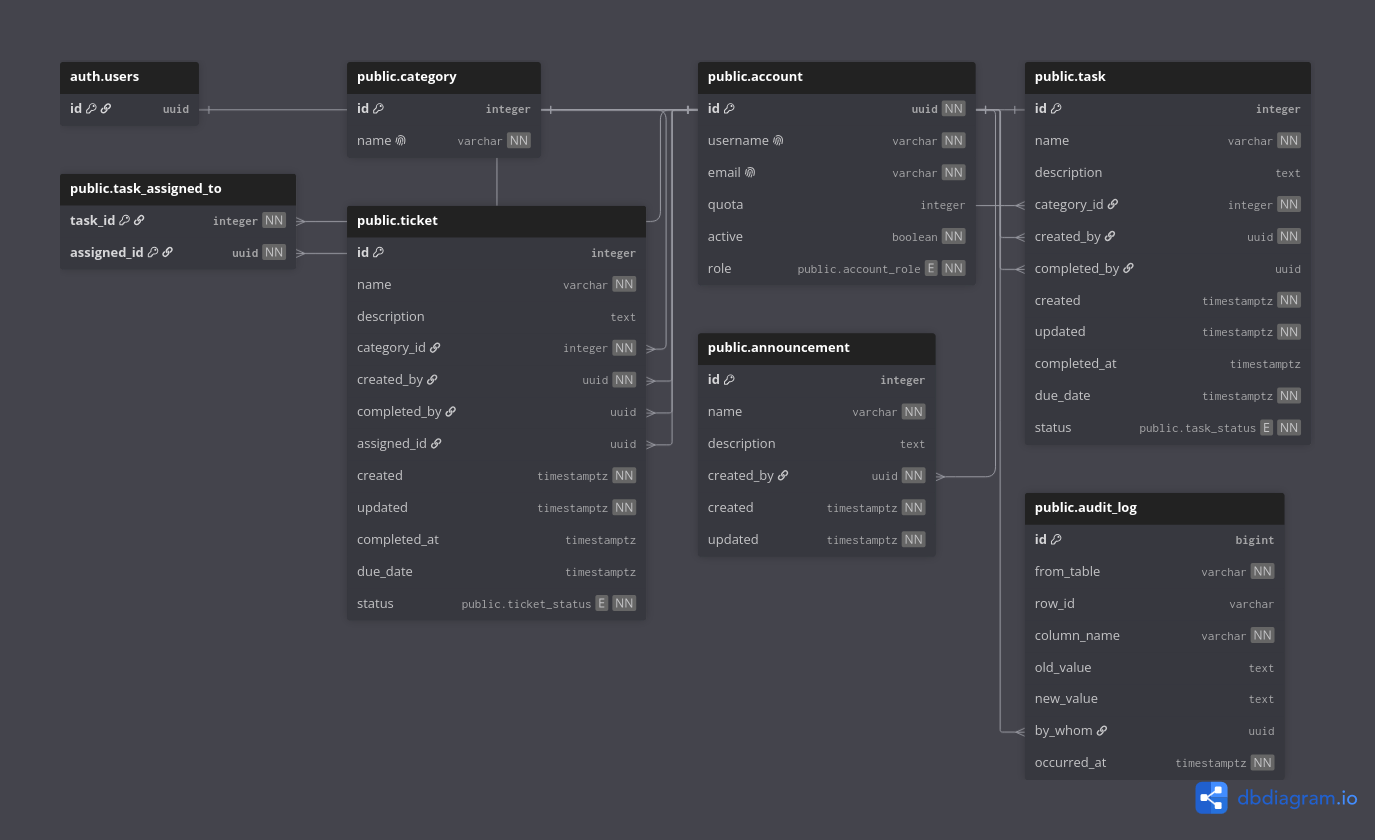
\includegraphics[width=0.95\textwidth]{model}
  \caption{Overview of database schema}
  \label{fig:model}
\end{figure}

\begin{table}[H]
  \footnotesize
  \begin{tabularx}{\textwidth}{@{}ll>{\RaggedRight\arraybackslash}X@{}}
    \toprule
    \textbf{Table} & \textbf{Primary key} & \textbf{Foreign keys} \\
    \midrule
    \texttt{account} & \texttt{id} (uuid) &
      \texttt{id} $\to$ \texttt{auth.users.id} \\
    \addlinespace[2pt]
    \texttt{category} & \texttt{id} (integer) & none \\
    \addlinespace[2pt]
    \texttt{ticket} & \texttt{id} (integer) &
      \texttt{category\_id} $\to$ \texttt{category.id};
      \texttt{created\_by}, \texttt{completed\_by}, \texttt{assigned\_id}
      $\to$ \texttt{account.id} \\
    \addlinespace[2pt]
    \texttt{task} & \texttt{id} (integer) &
      \texttt{category\_id} $\to$ \texttt{category.id};
      \texttt{created\_by}, \texttt{completed\_by} $\to$ \texttt{account.id} \\
    \addlinespace[2pt]
    \texttt{task\_assigned\_to} & (\texttt{task\_id}, \texttt{assigned\_id}) &
      \texttt{task\_id} $\to$ \texttt{task.id};
      \texttt{assigned\_id} $\to$ \texttt{account.id} \\
    \addlinespace[2pt]
    \texttt{announcement} & \texttt{id} (integer) &
      \texttt{created\_by} $\to$ \texttt{account.id} \\
    \addlinespace[2pt]
    \texttt{audit\_log} & \texttt{id} (bigint) &
      \texttt{by\_whom} $\to$ \texttt{account.id} \\
    \bottomrule
  \end{tabularx}
  \caption{Tables, keys and relationships}
  \label{tab:schema}
\end{table}

\begin{table}[H]
  \footnotesize
  \begin{tabularx}{\textwidth}{@{}ll>{\RaggedRight\arraybackslash}X@{}}
    \toprule
    \textbf{Enum type} & \textbf{Used by} & \textbf{Stored values} \\
    \midrule
    \texttt{account\_role} & \texttt{account.role} &
      \texttt{lab\_owner}, \texttt{lab\_admin}, \texttt{lab\_user} \\
    \addlinespace[2pt]
    \texttt{ticket\_status} & \texttt{ticket.status} &
      \texttt{pending}, \texttt{accept}, \texttt{reject} \\
    \addlinespace[2pt]
    \texttt{task\_status} & \texttt{task.status} &
      \texttt{in\_progress}, \texttt{complete} \\
    \bottomrule
  \end{tabularx}
  \caption{Enum types and the values actually stored in the column}
  \label{tab:enums}
\end{table}

\texttt{public.account(id, username, email, quota, active, role)} is the
application profile for an authenticated user. \texttt{id} is a uuid primary
key and foreign key to auth.users.id. \texttt{username} and \texttt{email} are
varchar not null. \texttt{quota} is an integer. \texttt{active} is a boolean
not null. \texttt{role} is an enum \texttt{public.account\_role} not null which
contains Lab Owner, Lab Admin and Lab user, stored as \texttt{lab\_owner},
\texttt{lab\_admin} and \texttt{lab\_user}.

\begin{note}
when checking just query the account by id and check if
role = \texttt{lab\_user}.
\end{note}

\texttt{public.category(id, name)} is a lookup table used to classify tickets
and tasks. \texttt{id} is an integer primary key and \texttt{name} is a varchar
not null.

\texttt{public.ticket(id, name, description, category\_id, created\_by,
completed\_by, assigned\_id, created, updated, completed\_at, due\_date,
status)} is a support ticket. \texttt{id} is an integer primary key.
\texttt{category\_id} is not null and a foreign key to category.id.
\texttt{created\_by} is not null and a foreign key to account.id.
\texttt{completed\_by} and \texttt{assigned\_id} are foreign keys to
account.id. \texttt{created} and \texttt{updated} are timestamptz not null.
\texttt{status} is an enum \texttt{public.ticket\_status} not null.

\begin{note}
you don't need to insert/update attributes created or updated since the
database will do that for you automatically.
\end{note}

\texttt{public.task(id, name, description, category\_id, created\_by,
completed\_by, created, updated, completed\_at, due\_date, status)} is a unit
of work optionally linked to a category. \texttt{id} is an integer primary key.
\texttt{category\_id} is not null and a foreign key to category.id.
\texttt{created\_by} is not null and a foreign key to account.id.
\texttt{completed\_by} is a foreign key to account.id. \texttt{created} and
\texttt{updated} are timestamptz not null. \texttt{status} is an enum
\texttt{public.task\_status} not null.

\begin{note}
date is the same as ticket.
\end{note}

\begin{note}[Clarify]
status in ticket could go from Pending $\to$ Accept/Reject while status in task
could only go from In-Progress to Complete. They are two separate enum types,
not one shared one.
\end{note}

\texttt{public.ticket\_status} is an enum which contains Pending, Accept and
Reject, stored as \texttt{pending}, \texttt{accept} and \texttt{reject}.

\texttt{public.task\_status} is an enum which contains In-Progress and
Complete, stored as \texttt{in\_progress} and \texttt{complete}.

\texttt{public.task\_assigned\_to(task\_id, assigned\_id)} is a join table
assigning accounts to tasks in a many to many relationship. \texttt{task\_id}
is a not null foreign key to task.id and \texttt{assigned\_id} is a not null
foreign key to account.id, together forming the primary key.

\texttt{public.announcement(id, name, description, created\_by, created,
updated)} is a broadcast message created by an account. \texttt{id} is an
integer primary key. \texttt{created\_by} is not null and a foreign key to
account.id. \texttt{created} and \texttt{updated} are timestamptz not null.

\texttt{public.audit\_log(id, from\_table, row\_id, column\_name, old\_value,
new\_value, by\_whom, occurred\_at)} is a change history recorded across
tables. \texttt{id} is a bigint primary key. \texttt{from\_table} and
\texttt{column\_name} are varchar not null. \texttt{row\_id} is a varchar.
\texttt{by\_whom} is a foreign key to account.id. \texttt{occurred\_at} is
timestamptz not null.

\begin{note}
this table is not filled in automatically, there is no trigger behind it, so
every endpoint that changes a row has to write its own audit rows.
\end{note}

\section{SqlAlchemy Class}

\begin{table}[H]
  \footnotesize
  \begin{tabularx}{\textwidth}{@{}l>{\RaggedRight\arraybackslash}X>{\RaggedRight\arraybackslash}X@{}}
    \toprule
    \textbf{Class} & \textbf{Defaults and constraints} &
    \textbf{Relationships} \\
    \midrule
    \texttt{Category} & none & \texttt{tasks}, \texttt{tickets} \\
    \addlinespace[3pt]
    \texttt{Account} &
      \texttt{role} defaults to \texttt{lab\_user}; \texttt{active} defaults to
      true; \texttt{quota} check $\geq$ 0; \texttt{username} and
      \texttt{email} unique; \texttt{id} cascades on delete &
      \texttt{tasks} and \texttt{tickets} created, completed and assigned;
      \texttt{announcements}; \texttt{audit\_entries} \\
    \addlinespace[3pt]
    \texttt{Task} &
      \texttt{status} defaults to \texttt{in\_progress}; \texttt{due\_date} not
      null; \texttt{category\_id} and \texttt{created\_by} restrict;
      \texttt{completed\_by} set null &
      \texttt{assignees}, many to many through \texttt{task\_assigned\_to} \\
    \addlinespace[3pt]
    \texttt{Ticket} &
      \texttt{status} defaults to \texttt{pending}; \texttt{due\_date}
      optional; \texttt{category\_id} and \texttt{created\_by} restrict;
      \texttt{completed\_by} and \texttt{assigned\_id} set null & none \\
    \addlinespace[3pt]
    \texttt{Announcement} & \texttt{created\_by} restrict & none \\
    \addlinespace[3pt]
    \texttt{AuditLog} &
      \texttt{by\_whom} set null; \texttt{occurred\_at} from the database &
      none \\
    \bottomrule
  \end{tabularx}
  \caption{ORM classes, every one mapping to the public table of the same name}
  \label{tab:orm}
\end{table}

\texttt{Category(id, name)} maps to public.category. \texttt{tasks} and
\texttt{tickets} are relationships back to Task and Ticket through their
\texttt{category\_id}.

\texttt{Account(id, username, email, role, quota, active)} maps to
public.account. \texttt{id} is a foreign key to auth.users.id with cascade on
delete. \texttt{username} and \texttt{email} are unique and not null.
\texttt{role} defaults to Lab user. \texttt{active} defaults to true.
\texttt{quota} has a check constraint requiring it to be greater than or equal
to zero. It also exposes relationships for tasks and tickets created,
completed, assigned, plus \texttt{announcements} and \texttt{audit\_entries}.

\texttt{Task(id, name, description, status, category\_id, created\_by,
completed\_by, created, updated, completed\_at, due\_date)} maps to public.task.
\texttt{status} defaults to In-Progress. \texttt{category\_id} and
\texttt{created\_by} are not null foreign keys with ondelete restrict.
\texttt{completed\_by} is a foreign key with ondelete set null.
\texttt{created} and \texttt{updated} are filled automatically by the database.
\texttt{due\_date} is not null. \texttt{assignees} is a many to many
relationship to Account through the \texttt{task\_assigned\_to} table.

\texttt{Ticket(id, name, description, status, category\_id, created\_by,
completed\_by, assigned\_id, created, updated, completed\_at, due\_date)} maps
to public.ticket. \texttt{status} defaults to Pending. \texttt{category\_id}
and \texttt{created\_by} are not null foreign keys with ondelete restrict.
\texttt{completed\_by} and \texttt{assigned\_id} are foreign keys with ondelete
set null. \texttt{created} and \texttt{updated} are filled automatically by the
database. \texttt{due\_date} is optional.

\texttt{Announcement(id, name, description, created\_by, created, updated)}
maps to public.announcement. \texttt{created\_by} is a not null foreign key
with ondelete restrict. \texttt{created} and \texttt{updated} are filled
automatically by the database.

\texttt{AuditLog(id, from\_table, row\_id, column\_name, old\_value,
new\_value, by\_whom, occurred\_at)} maps to \texttt{public.audit\_log}.
\texttt{id} is a bigint primary key. \texttt{from\_table} and
\texttt{column\_name} are not null. \texttt{by\_whom} is a foreign key with
ondelete set null. \texttt{occurred\_at} is filled automatically by the
database.

\texttt{TicketStatus}, \texttt{TaskStatus} and \texttt{AccountRole} are Python
string enums that back the \texttt{ticket\_status}, \texttt{task\_status} and
\texttt{account\_role} Postgres enum types, storing lowercase values such as
\texttt{in\_progress} rather than the member names.

\subsection{Additional Notes when query assignees}

Since \texttt{Task.assignees} is a collection (many to many through
\texttt{task\_assigned\_to}), you have to eager load it with
\texttt{selectinload}. On an async session the default lazy load cannot fire on
attribute access, so reading \texttt{task.assignees} without it raises
\texttt{MissingGreenlet}. \texttt{selectinload} also leaves the parent row count
alone, unlike \texttt{joinedload}, which repeats the Task row once per assignee.

\begin{code}
from sqlalchemy import select
from sqlalchemy.orm import selectinload

task = await session.scalar(
    select(Task).where(Task.id == task_id)
    .options(selectinload(Task.assignees))
)
\end{code}

That emits two queries, the second one loading the collection:

\begin{code}
SELECT ... FROM task WHERE task.id = 5;

SELECT ... FROM account
JOIN task_assigned_to
  ON account.id = task_assigned_to.assigned_id
WHERE task_assigned_to.task_id IN (5);
\end{code}

Without \texttt{.options(selectinload(Task.assignees))} there is no second
query at all, and touching \texttt{task.assignees} raises
\texttt{MissingGreenlet}.

Read more:
\url{https://docs.sqlalchemy.org/en/20/orm/queryguide/relationships.html#sqlalchemy.orm.selectinload}

\section{Ticket Endpoints}

\subsection{GET}

\texttt{GET /tickets} lists tickets. Every parameter is optional.

Scope comes first. An admin, meaning \texttt{lab\_admin} or
\texttt{lab\_owner}, sees every ticket. Everyone else sees only their own, the
rows where \texttt{created\_by} is their account id. Resolve the role with the
account lookup from section 1, then AND that filter onto every query, never OR,
and never let it come from a parameter. No parameter can widen it, which is why
\texttt{created\_by} is not one of them.

\begin{code}
SELECT * FROM ticket
 WHERE ((:is_admin AND NOT :only_owned)
        OR created_by = :caller_id)
   AND (:status IS NULL OR status = :status)
 ORDER BY created DESC
 LIMIT :limit
\end{code}

Parameters, all optional:

\begin{code}
GET /tickets
  ?ticket_id=41
  &status=pending
  &category_id=2
  &due_before=2026-10-01T00:00:00Z
  &only_owned=true
  &limit=20
\end{code}

There are six and no more: \texttt{ticket\_id}, \texttt{status},
\texttt{category\_id}, \texttt{due\_before}, \texttt{only\_owned} and
\texttt{limit}.

\texttt{ticket\_id} narrows to a single ticket and still goes through the scope
filter, so a \texttt{lab\_user} naming somebody else's ticket gets an empty page
rather than that ticket. \texttt{status} takes the stored lowercase value.
\texttt{category\_id} filters on the column directly. \texttt{due\_before} is an
upper bound on \texttt{due\_date}, and a ticket with a null due date falls out
of the results as soon as it is used. \texttt{only\_owned} is a boolean
defaulting to false. It lets an admin narrow the page to the tickets they
created themselves, instead of the whole table they would otherwise get. For a
\texttt{lab\_user} it changes nothing, they were already limited to their own,
so it is accepted and quietly does nothing rather than being an error. Note
which direction it runs, it only ever narrows the scope and never widens it,
which is what keeps it safe to take from a client at all. \texttt{limit}
defaults to 20 and caps at 100, and cap it rather than trusting it. There is no
sort parameter, the order is fixed at newest first.

An unknown parameter is an error, not something to ignore, since a dropped
filter looks like a filter that matched everything.

Response \texttt{200 OK}. \texttt{total} is the count before paging:

\begin{code}
{
  "items": [
    {
      "id": 41,
      "name": "Projector in Lab 3 wont turn on",
      "description": "No power LED",
      "category_id": 2,
      "created_by": "9f1c...e30a",
      "completed_by": null,
      "assigned_id": null,
      "status": "pending",
      "created": "2026-09-16T09:12:44.512Z",
      "updated": "2026-09-16T09:12:44.512Z",
      "completed_at": null,
      "due_date": "2026-09-30T17:00:00Z"
    }
  ],
  "total": 37,
  "limit": 20
}
\end{code}

No matches is an empty \texttt{items} with \texttt{total} zero, not a 404.

\texttt{GET /tickets/\{id\}} returns one ticket without the wrapper, same scope
rule. When a \texttt{lab\_user} asks for a ticket that exists but is not theirs,
answer \texttt{404}, not \texttt{403}. A 403 tells them it exists.

Reading writes nothing, no audit row, no quota, no \texttt{updated} bump.

Failure cases: \texttt{401} for a bad token, \texttt{403} when \texttt{active}
is false, \texttt{404} on a single ticket that does not exist or is out of
scope, \texttt{422} for a bad enum value, a bad number, a bad timestamp or an
unknown parameter, \texttt{500} otherwise without leaking the database error.

\begin{note}
own is written here as \texttt{created\_by} only. If a ticket can be assigned to
a \texttt{lab\_user}, make it
\texttt{created\_by = :caller\_id OR assigned\_id = :caller\_id}, or somebody
cannot see work assigned to them.
\end{note}

\subsection{POST}

\texttt{POST /tickets} creates a ticket. Requires a bearer token, and
\texttt{created\_by} always comes from that token, never from the body.

\begin{code}
{
  "name": "Projector in Lab 3 wont turn on",
  "description": "No power LED, tried two outlets",
  "category_id": 2,
  "assigned_id": null,
  "due_date": "2026-09-30T17:00:00Z"
}
\end{code}

\texttt{name} and \texttt{category\_id} are required, the rest are optional.
\texttt{category\_id} and \texttt{assigned\_id} must resolve to existing rows,
so check them yourself and give the caller a readable error instead of a foreign
key violation. \texttt{due\_date} is ISO 8601 with an offset.

Everything else is server side and a client may not send it. \texttt{id} is
generated, \texttt{created\_by} comes from the token, \texttt{status} is always
Pending on create, \texttt{created} and \texttt{updated} are filled by the
database, \texttt{completed\_by} and \texttt{completed\_at} stay null.

Quota. \texttt{account.quota} is a nullable integer spent one per ticket. Null
means no allowance configured, so unlimited, deduct nothing. Above zero is spent
by deducting one. Zero means refused and no ticket row is written. Deduct with a
conditional update rather than reading the value and writing it back, otherwise
two requests arriving together both read the same number and drive the column to
-1, which the check constraint rejects:

\begin{code}
UPDATE account
   SET quota = quota - 1
 WHERE id = :caller_id
   AND quota > 0
RETURNING quota;
\end{code}

A row back means the deduction took, nothing back means the quota was already
zero. A deduction is not refunded when a ticket is later rejected, so quota
counts tickets opened rather than tickets outstanding.

Audit. Nothing writes \texttt{audit\_log} for you, there is no trigger, so a
change is recorded only if the endpoint inserts it. The table is column
oriented, \texttt{column\_name} is not null, so one row is one changed column.
\texttt{row\_id} is a varchar and not a real foreign key, which is what lets it
hold an integer ticket.id and a uuid account.id, so stringify whichever key you
mean. \texttt{old\_value} and \texttt{new\_value} are text. \texttt{by\_whom} is
the caller. \texttt{occurred\_at} is filled by the database.

\begin{code}
INSERT INTO audit_log
  (from_table, row_id, column_name,
   old_value, new_value, by_whom)
VALUES
  ('ticket', '41', 'status',
   NULL, 'pending', :caller_id),
  ('account', :caller_id, 'quota',
   '5', '4', :caller_id);
\end{code}

The ticket insert, the quota update and the audit rows go in one transaction,
they commit together or not at all.

Response \texttt{201 Created} returns the new row in the same shape as GET, with
\texttt{status} as the stored lowercase \texttt{pending}.

Failure cases: \texttt{401} for a bad token, \texttt{403} when \texttt{active}
is false or the role may not set a field that was sent, \texttt{403} with the
body below when the quota is exhausted, \texttt{422} when \texttt{name} or
\texttt{category\_id} is missing, a timestamp will not parse, a foreign key does
not resolve or a server side field was supplied, \texttt{500} otherwise without
leaking the database error.

\begin{code}
{
  "detail": "Ticket quota exhausted",
  "code": "quota_exhausted",
  "quota": 0
}
\end{code}

\begin{note}
a \texttt{lab\_user} raising their own ticket probably should not choose
\texttt{assigned\_id}, while an admin should. If you want that rule, check the
role and drop the field for a \texttt{lab\_user}.
\end{note}

\subsection{POST migrate to PATCH}

\texttt{PATCH /tickets/\{id\}} updates part of a ticket. Same auth as POST.

\begin{note}
there is no PUT here and that is deliberate. PUT means replace the whole row, so
a client sending only \texttt{status} would null out the description and the due
date along with it. Updates on a ticket are partial, which is what PATCH means.
If you were expecting PUT in the route table it is not missing, it is this.
\end{note}

Only the fields being changed go in the body. A field left out is untouched, so
accepting a ticket is a body with \texttt{status} in it and nothing else. An
empty body is a bad request rather than a successful no-op.

\begin{code}
{
  "assigned_id": "4b7d...91cc",
  "status": "accept"
}
\end{code}

Left out and sent as null are different instructions. Out means do not touch.
Null means clear, and that only works on \texttt{description},
\texttt{assigned\_id} and \texttt{due\_date}, the nullable columns. Null for
\texttt{name}, \texttt{category\_id} or \texttt{status} is a validation error.

\texttt{id}, \texttt{created\_by} and \texttt{created} are immutable, so reject
an attempt to change them rather than ignoring it. \texttt{updated} is refreshed
by the database. \texttt{completed\_by} and \texttt{completed\_at} are derived,
never taken from the body.

Status goes from Pending to Accept or Reject and that is the only move there is.
Both are terminal, an accepted ticket cannot later be rejected and a rejected
one cannot be reopened. Anything else is refused. Editing a Pending ticket while
leaving \texttt{status} as Pending is just an edit.

When the status leaves Pending, set \texttt{completed\_by} to the caller and
\texttt{completed\_at} to now. A rejected ticket counts as completed, the column
records who closed it, not who agreed with it.

Guard the transition with the old status in the where clause, the same way the
quota deduction is guarded, so two admins pressing accept and reject at the same
moment cannot both win:

\begin{code}
UPDATE ticket
   SET status = 'accept',
       completed_by = :caller_id,
       completed_at = now()
 WHERE id = :ticket_id
   AND status = 'pending'
RETURNING id;
\end{code}

No row back means somebody already closed it, so return the conflict rather than
reporting success.

Quota is untouched here, it is spent on open and not refunded on reject.

The audit matters more here than on POST because now there are real previous
values. Write one row per column that actually changed, with both
\texttt{old\_value} and \texttt{new\_value} filled. A field that was sent but
already held that value is not a change, do not write a row for it.

\begin{code}
INSERT INTO audit_log
  (from_table, row_id, column_name,
   old_value, new_value, by_whom)
VALUES
  ('ticket', '41', 'status',
   'pending', 'accept', :caller_id),
  ('ticket', '41', 'assigned_id',
   NULL, '4b7d...91cc', :caller_id);
\end{code}

Same transaction as the update, and again nothing writes them for you.

Response \texttt{200 OK} returns the updated row in the same shape as GET.

Failure cases: \texttt{401} for a bad token, \texttt{403} when \texttt{active}
is false or the role may not make this change, \texttt{404} when no ticket has
that id, \texttt{409} with the body below when the transition is not legal or
another request closed the ticket first, \texttt{422} for the POST body problems
plus an empty body, a null on a not null column, or an attempt to write an
immutable or derived field, \texttt{500} otherwise.

\begin{code}
{
  "detail": "Ticket is already accept",
  "code": "invalid_status_transition",
  "from": "accept",
  "to": "reject"
}
\end{code}

\begin{note}[Additional note on roles]
the rule I would expect is a \texttt{lab\_user} editing the wording of their own
Pending ticket and nothing else, with accept, reject and assign belonging to
\texttt{lab\_admin} and \texttt{lab\_owner}, and nobody accepting a ticket they
opened themselves. That is policy rather than schema, so confirm it.
\end{note}

\section{Task Endpoints}

Tasks work like tickets, so this section covers only what is different. Auth,
the error bodies, the one transaction rule and the audit mechanics are all the
same as section 3.

Three differences drive the rest. A task has no \texttt{assigned\_id} column,
assignment lives in the many to many \texttt{task\_assigned\_to}, so assignees
are a list rather than a field. \texttt{due\_date} is not null on a task, where
on a ticket it was optional. And \texttt{task\_status} only goes
\texttt{in\_progress} $\to$ \texttt{complete}, there is no pending, accept or
reject, so there is nothing to approve here, only work to finish.

\subsection{GET}

\texttt{GET /tasks} lists tasks. Every parameter is optional.

Scope is wider than it was for tickets. An admin sees every task. Everyone else
sees the tasks they created and the tasks they are assigned, and that second
half is the whole reason the join table exists, so it cannot be left out:

\begin{code}
SELECT t.* FROM task t
 WHERE ((:is_admin AND NOT :only_owned)
        OR t.created_by = :caller_id
        OR EXISTS (SELECT 1
                     FROM task_assigned_to a
                    WHERE a.task_id = t.id
                      AND a.assigned_id = :caller_id))
 ORDER BY t.created DESC
 LIMIT :limit
\end{code}

The parameters are the six from section 3.1 with \texttt{task\_id} in place of
\texttt{ticket\_id}, and \texttt{status} here takes \texttt{in\_progress} or
\texttt{complete}. \texttt{only\_owned} means the same thing but covers both
halves of the wider scope, so an admin setting it gets the tasks they created
and the tasks they are assigned, not just the ones they created.

Each task comes back with an \texttt{assignees} array of account ids, which is
the one field tickets do not have:

\begin{code}
{
  "id": 88,
  "name": "Re-image the lab 2 machines",
  "description": "Ubuntu 24.04, standard image",
  "category_id": 3,
  "created_by": "9f1c...e30a",
  "completed_by": null,
  "assignees": ["4b7d...91cc", "7a02...b511"],
  "status": "in_progress",
  "created": "2026-09-16T09:12:44.512Z",
  "updated": "2026-09-16T09:12:44.512Z",
  "completed_at": null,
  "due_date": "2026-09-30T17:00:00Z"
}
\end{code}

Load that array with \texttt{selectinload}, as section 2.1 says. On a list
endpoint it costs one extra query for the whole page rather than one per task,
and it is not optional on an async session, a lazy load there raises
\texttt{MissingGreenlet} rather than quietly working.

\subsection{POST}

\texttt{POST /tasks} creates a task. \texttt{created\_by} comes from the token
as always.

\begin{code}
{
  "name": "Re-image the lab 2 machines",
  "description": "Ubuntu 24.04, standard image",
  "category_id": 3,
  "due_date": "2026-09-30T17:00:00Z",
  "assignees": ["4b7d...91cc", "7a02...b511"]
}
\end{code}

\texttt{name}, \texttt{category\_id} and \texttt{due\_date} are all required.
The required due date is the difference from POST on a ticket, the column is not
null so there is no creating a task without one.

\texttt{assignees} is a list of account ids and may be empty or absent, which
creates an unassigned task. Every id in it must exist, so check them in one
query rather than one per id, and reject the whole request if any fails rather
than creating the task with the assignees that happened to resolve. Repeated ids
are not an error but they are also not two rows, the pair is the primary key of
\texttt{task\_assigned\_to}, so collapse them before inserting or the insert
fails on the duplicate.

\texttt{status} is always \texttt{in\_progress} on create, a client cannot open a
task that is already complete. \texttt{completed\_by} and \texttt{completed\_at}
stay null.

Quota is not touched here. It is spent per ticket, and nothing in section 1 ties
it to tasks. If tasks are meant to cost quota as well then say so and it becomes
the same conditional update as in section 3.2, but as written a task is free.

The audit needs a row per populated task column, then one more per assignee, and
those point at the join table rather than at the task:

\begin{code}
INSERT INTO audit_log
  (from_table, row_id, column_name,
   old_value, new_value, by_whom)
VALUES
  ('task', '88', 'status',
   NULL, 'in_progress', :caller_id),
  ('task_assigned_to', '88', 'assigned_id',
   NULL, '4b7d...91cc', :caller_id);
\end{code}

\texttt{row\_id} here is the task id, since that is what identifies the row
people will search for later. The task insert, the \texttt{task\_assigned\_to}
inserts and the audit rows are one transaction.

Response \texttt{201 Created} returns the task in the shape above, assignees
included.

Failure cases are those of section 3.2, minus the quota case, plus \texttt{422}
when \texttt{due\_date} is missing or when an id in \texttt{assignees} does not
resolve to an account.

\subsection{PATCH}

\texttt{PATCH /tasks/\{id\}} updates part of a task. Partial body, same omitted
versus null rule as section 3.3.

\texttt{due\_date} is the exception to that rule. It can be changed but it
cannot be cleared, because the column is not null, so a null there is a
validation error rather than a way to remove a deadline.

Status goes \texttt{in\_progress} $\to$ \texttt{complete} and that is the only
move. Complete is terminal, a finished task does not go back to in progress.
Guard it with the old status in the where clause exactly as section 3.3 does,
and set \texttt{completed\_by} and \texttt{completed\_at} when the status leaves
\texttt{in\_progress}:

\begin{code}
UPDATE task
   SET status = 'complete',
       completed_by = :caller_id,
       completed_at = now()
 WHERE id = :task_id
   AND status = 'in_progress'
RETURNING id;
\end{code}

\texttt{assignees} is the awkward one, because a list has no partial form.
Leaving it out means do not touch the assignments. Sending it means replace the
whole set with what was sent, so sending an empty list unassigns everybody.
There is no way to add one person without naming the others, and if you want
that it needs its own endpoint rather than a special case here.

That replacement is a set difference, not a delete and reinsert. Work out which
ids were added and which were removed, apply only those, and leave the unchanged
rows alone. Reinserting a row that was already there gives you a primary key
violation and, worse, an audit trail saying somebody was unassigned and
reassigned when nothing actually happened to them.

Audit one row per added or removed assignee, with the direction carried by which
side is null:

\begin{code}
INSERT INTO audit_log
  (from_table, row_id, column_name,
   old_value, new_value, by_whom)
VALUES
  ('task_assigned_to', '88', 'assigned_id',
   NULL, '3c55...02af', :caller_id),
  ('task_assigned_to', '88', 'assigned_id',
   '7a02...b511', NULL, :caller_id);
\end{code}

A null \texttt{old\_value} is an assignment, a null \texttt{new\_value} is an
unassignment.

Response \texttt{200 OK} returns the updated task with its assignees. Failure
cases are those of section 3.3, with \texttt{409} covering the in progress to
complete transition and \texttt{422} covering a null \texttt{due\_date} or an
assignee id that does not resolve.

\begin{note}[Additional note on roles]
assigning people and completing a task read like admin actions, but a
\texttt{lab\_user} marking their own assigned task complete is the normal way
this gets used. Decide whether an assignee may complete their own task, it is
the one permission here that is not obvious.
\end{note}

\end{document}
